% =====================================================================
%  Artigo: Caixeiro Viajante (berlin52) - branch and bound x guloso
%
%  Como usar no Overleaf:
%    New Project > Upload Project > escolha o arquivo artigo_overleaf.zip
%    Compilador: pdfLaTeX (o padrão do Overleaf)
%
%  O que está em VERMELHO e entre colchetes no PDF precisa ser preenchido
%  (nomes do grupo, instituição, professor). Procure por \pendente.
% =====================================================================
\documentclass[12pt,a4paper]{article}

\usepackage[T1]{fontenc}
\usepackage[utf8]{inputenc}
\usepackage[english,brazil]{babel}
\usepackage{amsmath}
\usepackage{newtxtext,newtxmath}
\usepackage[a4paper,top=3cm,left=3cm,bottom=2cm,right=2cm]{geometry}
\usepackage{microtype}
\usepackage{graphicx}
\usepackage{booktabs}
\usepackage{xcolor}
\usepackage{enumitem}
\usepackage{tikz}
\usetikzlibrary{babel}
\usepackage[font=small,labelfont=bf]{caption}
\usepackage{subcaption}
\usepackage{algorithm}
\usepackage[noend]{algpseudocode}
\usepackage[hidelinks]{hyperref}

\graphicspath{{figuras/}}

% Evita avisos de links duplicados nas linhas numeradas dos pseudocódigos
\makeatletter
\providecommand{\theHALG@line}{}
\renewcommand{\theHALG@line}{\thealgorithm.\arabic{ALG@line}}
\makeatother

% Campos a preencher aparecem em vermelho no PDF
\newcommand{\pendente}[1]{\textcolor{red}{[#1]}}
% Nomes de variáveis nos pseudocódigos
\newcommand{\algvar}[1]{\textit{#1}}

% Pseudocódigo em português
\floatname{algorithm}{Algoritmo}
\algrenewcommand\algorithmicrequire{\textbf{Entrada:}}
\algrenewcommand\algorithmicensure{\textbf{Saída:}}
\algrenewcommand\algorithmicfunction{\textbf{função}}
\algrenewcommand\algorithmicprocedure{\textbf{procedimento}}
\algrenewcommand\algorithmicwhile{\textbf{enquanto}}
\algrenewcommand\algorithmicfor{\textbf{para}}
\algrenewcommand\algorithmicdo{\textbf{faça}}
\algrenewcommand\algorithmicif{\textbf{se}}
\algrenewcommand\algorithmicthen{\textbf{então}}
\algrenewcommand\algorithmicelse{\textbf{senão}}
\algrenewcommand\algorithmicreturn{\textbf{retorne}}
\algrenewcommand\algorithmicend{\textbf{fim}}

\title{O Problema do Caixeiro Viajante na instância berlin52:\\
\emph{branch and bound} versus a heurística do vizinho mais próximo}

\author{%
  Álisson \pendente{sobrenome} \quad \pendente{Integrante 2} \quad \pendente{Integrante 3}\\[6pt]
  \normalsize \pendente{Curso} --- \pendente{Instituição}\\
  \normalsize Projeto e Análise de Algoritmos --- Prof.\ \pendente{nome do professor}%
}

\date{Novembro de 2026}

\begin{document}

\maketitle

\begin{abstract}
Este trabalho compara dois algoritmos para o Problema do Caixeiro Viajante (PCV) simétrico: um algoritmo exato de \emph{branch and bound} (B\&B), que usa como limite inicial o custo de uma rota gulosa, e a heurística gulosa do vizinho mais próximo. Os dois algoritmos foram modelados, analisados quanto à complexidade de tempo e de espaço e implementados em Python. Os experimentos usaram a instância berlin52 da TSPLIB e sub-instâncias formadas pelas suas $n$ primeiras cidades. O B\&B encontrou a rota ótima para até 13 cidades, caso em que levou cerca de 10\,s e visitou apenas 1,7\% dos nós da árvore de busca completa; seu tempo cresceu, em média, 4,4 vezes a cada cidade acrescentada. O guloso resolveu as 52 cidades em 0,15\,ms, com tempo compatível com a previsão $\Theta(n^2)$, mas produziu rotas de 5\% a 19\% mais caras que a ótima: na instância completa, custo 8980 contra o ótimo conhecido de 7542.

\medskip
\noindent\textbf{Palavras-chave:} caixeiro viajante; \emph{branch and bound}; heurística gulosa; vizinho mais próximo; análise de algoritmos.
\end{abstract}

\begin{otherlanguage}{english}
\begin{abstract}
This paper compares two algorithms for the symmetric Traveling Salesman Problem (TSP): an exact branch-and-bound (B\&B) algorithm, initialized with the cost of a greedy tour as its upper bound, and the nearest-neighbor greedy heuristic. Both algorithms were modeled, analyzed for worst-case time and space complexity, and implemented in Python. Experiments used the berlin52 instance from TSPLIB and sub-instances formed by its first $n$ cities. B\&B found optimal tours for up to 13 cities, taking about 10\,s and visiting only 1.7\% of the nodes of the full search tree; its running time grew on average 4.4 times per added city. The greedy heuristic solved all 52 cities in 0.15\,ms, consistent with its $\Theta(n^2)$ bound, but its tours were 5\% to 19\% longer than optimal: 8980 against the known optimum of 7542 on the full instance.

\medskip
\noindent\textbf{Keywords:} traveling salesman; branch and bound; greedy heuristic; nearest neighbor; analysis of algorithms.
\end{abstract}
\end{otherlanguage}

% =====================================================================
\section{Introdução}
% =====================================================================

O Problema do Caixeiro Viajante (PCV) consiste em, dado um conjunto de cidades e as distâncias entre cada par delas, encontrar a rota de menor custo que visita cada cidade exatamente uma vez e retorna à cidade de origem. Apesar do enunciado simples, o PCV é um dos problemas de otimização combinatória mais estudados~\cite{applegate2006}, tanto pelas aplicações (roteamento de veículos, perfuração de placas de circuito, sequenciamento de tarefas) quanto por ser um representante clássico dos problemas NP-difíceis~\cite{karp1972,garey1979}.

A dificuldade está no tamanho do espaço de soluções: com $n$ cidades há $(n-1)!/2$ rotas distintas. Para as 52 cidades da instância berlin52, isso dá cerca de $7{,}8 \times 10^{65}$ rotas, o que torna inviável qualquer enumeração completa. Há, então, dois caminhos: algoritmos exatos que evitam explorar boa parte do espaço, mas mantêm tempo exponencial no pior caso, e heurísticas, que são rápidas mas não garantem a melhor rota.

Este artigo, desenvolvido conforme o enunciado do trabalho prático da disciplina~\cite{enunciado}, compara um representante de cada abordagem: um \emph{branch and bound} (B\&B), algoritmo exato baseado em busca exaustiva com \emph{backtracking} e poda, e a heurística gulosa do vizinho mais próximo. Para cada um, apresentamos o pseudocódigo, o paradigma de projeto e a complexidade de tempo e de espaço no pior caso, além de um argumento de corretude para o B\&B e de um contraexemplo de otimalidade para o guloso. Em seguida, medimos o tempo de execução e a qualidade das rotas na instância berlin52~\cite{reinelt1991} e em sub-instâncias dela, e comparamos os resultados com a teoria.

O texto está organizado assim: a Seção~\ref{sec:modelagem} apresenta a modelagem do problema; a Seção~\ref{sec:algoritmos}, os algoritmos e sua análise; a Seção~\ref{sec:implementacao}, as decisões de implementação; a Seção~\ref{sec:experimentos}, os experimentos; a Seção~\ref{sec:discussao} discute os resultados; e a Seção~\ref{sec:conclusao} conclui.

% =====================================================================
\section{Modelagem do problema}\label{sec:modelagem}
% =====================================================================

Modelamos o PCV como um grafo completo, não direcionado e ponderado $G = (V, E)$, em que $V = \{1, \dots, n\}$ é o conjunto de cidades e cada aresta $\{i, j\} \in E$ tem peso $d_{ij} \ge 0$, a distância entre as cidades $i$ e $j$. Como $d_{ij} = d_{ji}$, o problema é simétrico.

\paragraph{Entrada.} Um conjunto de $n$ cidades, cada uma com coordenadas $(x_i, y_i)$ no plano. Na berlin52, as coordenadas não são geográficas: são posições em um plano, com unidade arbitrária. As distâncias seguem a convenção \texttt{EUC\_2D} da TSPLIB~\cite{reinelt1991}, isto é, a distância euclidiana arredondada para o inteiro mais próximo:
\[
  d_{ij} = \left\lfloor \sqrt{(x_i - x_j)^2 + (y_i - y_j)^2} + 0{,}5 \right\rfloor .
\]
Esse arredondamento é necessário para reproduzir o ótimo oficial da instância, 7542.

\paragraph{Saída.} Uma permutação $\pi = (\pi_1, \pi_2, \dots, \pi_n)$ das cidades, que representa o ciclo $\pi_1 \to \pi_2 \to \dots \to \pi_n \to \pi_1$, ou seja, um ciclo hamiltoniano de $G$.

\paragraph{Função objetivo.} Minimizar o custo total do ciclo, incluindo a aresta de volta à cidade inicial:
\[
  \min_{\pi} \; C(\pi) = \sum_{k=1}^{n-1} d_{\pi_k \pi_{k+1}} + d_{\pi_n \pi_1} .
\]

\paragraph{Representação do grafo.} Usamos uma matriz de adjacência $D$ de dimensão $n \times n$, com $D[i][j] = d_{ij}$, calculada uma única vez antes da execução dos algoritmos. A escolha se justifica por três motivos: (i) o grafo é completo, com $n(n-1)/2$ arestas, de modo que uma lista de adjacência não economizaria memória; (ii) os dois algoritmos consultam distâncias no laço mais interno, e a matriz responde cada consulta em tempo $O(1)$, sem recalcular raízes quadradas; e (iii) o custo de memória é pequeno: $52^2 = 2704$ inteiros para a berlin52.

\paragraph{Espaço de soluções.} Há $n!$ permutações, mas cada ciclo é representado por $n$ delas (uma para cada cidade de partida) e pode ser percorrido em dois sentidos. O número de rotas distintas é, portanto,
\[
  \frac{n!}{2n} = \frac{(n-1)!}{2},
\]
o que dá 181.440 rotas para $n = 10$, cerca de $2{,}4 \times 10^{8}$ para $n = 13$ e cerca de $7{,}8 \times 10^{65}$ para $n = 52$.

\paragraph{Classe de complexidade.} A versão de decisão do PCV (``existe um ciclo de custo no máximo $k$?'') é NP-completa, por redução a partir do problema do ciclo hamiltoniano~\cite{karp1972,garey1979}; a versão de otimização, tratada aqui, é NP-difícil. O problema continua NP-difícil mesmo quando restrito a pontos no plano com distância euclidiana~\cite{papadimitriou1977}, que é o caso da berlin52. Assim, não se conhece algoritmo exato de tempo polinomial para ele, e a existência de um implicaria P = NP.

% =====================================================================
\section{Algoritmos}\label{sec:algoritmos}
% =====================================================================

Esta seção apresenta os dois algoritmos. Para cada um, descrevemos a ideia, o pseudocódigo, o paradigma de projeto e a complexidade de tempo e de espaço no pior caso, em função do número de cidades $n$ e com a notação assintótica usual~\cite{cormen2009}.

\subsection{Heurística gulosa: vizinho mais próximo}\label{sec:guloso}

\paragraph{Ideia.} Partindo de uma cidade inicial, o algoritmo vai sempre para a cidade ainda não visitada mais próxima da cidade atual. Quando todas as cidades foram visitadas, a rota é fechada com a aresta de volta à cidade inicial. O Algoritmo~\ref{alg:guloso} apresenta o pseudocódigo; em caso de empate, vence a cidade de menor índice.

\begin{algorithm}[htbp]
\caption{Vizinho mais próximo (guloso)}
\label{alg:guloso}
\begin{algorithmic}[1]
\Require matriz de distâncias $D$ ($n \times n$) e cidade inicial $s$
\Ensure uma rota que visita cada cidade exatamente uma vez
\Function{Guloso}{$D, s$}
  \State $\algvar{rota} \gets [s]$; \ $\algvar{visitada}[1..n] \gets \textsc{falso}$; \ $\algvar{visitada}[s] \gets \textsc{verdadeiro}$
  \While{$|\algvar{rota}| < n$}
    \State $\algvar{atual} \gets$ último elemento de $\algvar{rota}$
    \State $\algvar{prox} \gets \textsc{nulo}$
    \For{$j \gets 1$ \textbf{até} $n$}
      \If{\textbf{não} $\algvar{visitada}[j]$ \textbf{e} ($\algvar{prox} = \textsc{nulo}$ \textbf{ou} $D[\algvar{atual}][j] < D[\algvar{atual}][\algvar{prox}]$)}
        \State $\algvar{prox} \gets j$
      \EndIf
    \EndFor
    \State acrescente $\algvar{prox}$ ao fim de $\algvar{rota}$; \ $\algvar{visitada}[\algvar{prox}] \gets \textsc{verdadeiro}$
  \EndWhile
  \State \Return $\algvar{rota}$ \Comment{a volta para $s$ entra no cálculo do custo}
\EndFunction
\end{algorithmic}
\end{algorithm}

\paragraph{Paradigma.} Guloso: a cada passo, o algoritmo faz a escolha localmente ótima (a aresta mais curta disponível a partir da cidade atual) e nunca revê uma escolha já feita. Não há retrocesso nem qualquer consideração sobre os passos seguintes.

\paragraph{Complexidade.} O laço \textbf{enquanto} executa $n - 1$ iterações e, em cada uma, o laço \textbf{para} percorre as $n$ cidades, com custo $O(1)$ por cidade graças à matriz. O tempo é, portanto, $\Theta(n^2)$, tanto no pior quanto no melhor caso. Quanto ao espaço, o algoritmo usa $\Theta(n)$ de memória adicional (os vetores \algvar{rota} e \algvar{visitada}), além da matriz de distâncias, que ocupa $\Theta(n^2)$ e é compartilhada pelos dois algoritmos. A construção da matriz também custa $\Theta(n^2)$ e é feita uma única vez.

\paragraph{Contraexemplo.} O vizinho mais próximo sempre produz uma rota válida, mas não necessariamente a ótima. As quatro primeiras cidades da berlin52 bastam para mostrar isso (Figura~\ref{fig:contraexemplo}). Partindo da cidade~1, o guloso escolhe a cidade~3 (distância 281, a menor), depois a cidade~4 (604, menor que os 649 até a cidade~2) e, por fim, a cidade~2, a única restante. Como a cidade~2 fica no canto oposto, essa última escolha é forçada a usar a aresta $4 \to 2$, de comprimento 1047, e a rota custa $281 + 604 + 1047 + 666 = 2598$. A rota ótima, $1 \to 2 \to 3 \to 4 \to 1$, custa $666 + 649 + 604 + 396 = 2315$: ela começa justamente pela aresta mais longa que sai da cidade~1, que o guloso evita, e o guloso fica 12,2\% acima dela.

\begin{figure}[htbp]
\centering
\begin{subfigure}[b]{0.48\linewidth}
\centering
\begin{tikzpicture}[x=0.006cm, y=0.006cm, >=stealth,
    cidade/.style={circle, fill=black, inner sep=0pt, minimum size=5pt},
    dist/.style={midway, fill=white, inner sep=1pt, font=\scriptsize}]
  \node[cidade, label={[font=\small]below:1}] (c1) at (565,575) {};
  \node[cidade, label={[font=\small]left:2}]  (c2) at (25,185)  {};
  \node[cidade, label={[font=\small]above:3}] (c3) at (345,750) {};
  \node[cidade, label={[font=\small]right:4}] (c4) at (945,685) {};
  \draw[->, thick, red!75!black] (c1) -- node[dist] {281}  (c3);
  \draw[->, thick, red!75!black] (c3) -- node[dist] {604}  (c4);
  \draw[->, thick, red!75!black] (c4) -- node[dist] {1047} (c2);
  \draw[->, thick, red!75!black] (c2) -- node[dist] {666}  (c1);
\end{tikzpicture}
\caption{Guloso: $1 \to 3 \to 4 \to 2 \to 1$, custo 2598.}
\end{subfigure}
\hfill
\begin{subfigure}[b]{0.48\linewidth}
\centering
\begin{tikzpicture}[x=0.006cm, y=0.006cm, >=stealth,
    cidade/.style={circle, fill=black, inner sep=0pt, minimum size=5pt},
    dist/.style={midway, fill=white, inner sep=1pt, font=\scriptsize}]
  \node[cidade, label={[font=\small]below:1}] (c1) at (565,575) {};
  \node[cidade, label={[font=\small]left:2}]  (c2) at (25,185)  {};
  \node[cidade, label={[font=\small]above:3}] (c3) at (345,750) {};
  \node[cidade, label={[font=\small]right:4}] (c4) at (945,685) {};
  \draw[->, thick, green!50!black] (c1) -- node[dist] {666} (c2);
  \draw[->, thick, green!50!black] (c2) -- node[dist] {649} (c3);
  \draw[->, thick, green!50!black] (c3) -- node[dist] {604} (c4);
  \draw[->, thick, green!50!black] (c4) -- node[dist] {396} (c1);
\end{tikzpicture}
\caption{Ótima: $1 \to 2 \to 3 \to 4 \to 1$, custo 2315.}
\end{subfigure}
\caption{Contraexemplo de otimalidade do vizinho mais próximo com as quatro primeiras cidades da berlin52, desenhadas nas suas coordenadas reais. Os números nas arestas são as distâncias.}
\label{fig:contraexemplo}
\end{figure}

Em geral, o vizinho mais próximo não tem garantia de aproximação constante: para instâncias que satisfazem a desigualdade triangular, a razão entre o custo obtido e o ótimo é limitada por $O(\log n)$, e existem instâncias em que essa razão de fato cresce de forma logarítmica~\cite{rosenkrantz1977}.

\subsection{Algoritmo exato: \emph{branch and bound}}\label{sec:bnb}

\paragraph{Ideia.} O algoritmo constrói as rotas cidade a cidade, explorando em profundidade uma árvore de espaço de estados: a raiz é a cidade~1, e cada nó no nível $k$ representa um caminho parcial com $k + 1$ cidades. Cada nó é ramificado (\emph{branch}) em um filho para cada cidade ainda não visitada. Ao chegar a um nó, o algoritmo compara o custo do caminho parcial com o da melhor rota completa conhecida e, se o primeiro já for maior ou igual, descarta toda a subárvore (\emph{bound}). Duas decisões aumentam a poda: a cidade~1 é fixada como ponto de partida, o que elimina as rotações de um mesmo ciclo; e a melhor rota inicial é a do vizinho mais próximo, o que permite podar desde o primeiro ramo, sem esperar pela primeira rota completa. O Algoritmo~\ref{alg:bnb} apresenta o pseudocódigo.

\begin{algorithm}[htbp]
\caption{\emph{Branch and bound} com limite inicial dado pelo guloso}
\label{alg:bnb}
\begin{algorithmic}[1]
\Require matriz de distâncias $D$ ($n \times n$)
\Ensure uma rota de custo mínimo e o seu custo
\Function{BranchAndBound}{$D$}
  \State $\algvar{melhorRota} \gets{}$ \Call{Guloso}{$D, 1$}
  \State $\algvar{melhorCusto} \gets{}$ \Call{Custo}{$\algvar{melhorRota}$}
  \State $\algvar{rota} \gets [1]$; \ $\algvar{visitada}[1] \gets \textsc{verdadeiro}$ (demais: \textsc{falso})
  \State \Call{Explorar}{$0$}
  \State \Return $(\algvar{melhorRota}, \algvar{melhorCusto})$
\EndFunction
\Statex
\Procedure{Explorar}{$c$} \Comment{$c$: custo do caminho parcial em \algvar{rota}}
  \If{$c \ge \algvar{melhorCusto}$}
    \State \Return \Comment{poda (\emph{bound})}
  \EndIf
  \If{$|\algvar{rota}| = n$}
    \State $\algvar{total} \gets c + D[\text{último de } \algvar{rota}][1]$ \Comment{fecha o ciclo}
    \If{$\algvar{total} < \algvar{melhorCusto}$}
      \State $\algvar{melhorCusto} \gets \algvar{total}$; \ $\algvar{melhorRota} \gets$ cópia de $\algvar{rota}$
    \EndIf
    \State \Return
  \EndIf
  \State $\algvar{atual} \gets$ último elemento de $\algvar{rota}$
  \For{$v \gets 1$ \textbf{até} $n$} \Comment{ramificação (\emph{branch})}
    \If{\textbf{não} $\algvar{visitada}[v]$}
      \State acrescente $v$ ao fim de $\algvar{rota}$; \ $\algvar{visitada}[v] \gets \textsc{verdadeiro}$
      \State \Call{Explorar}{$c + D[\algvar{atual}][v]$}
      \State remova $v$ de $\algvar{rota}$; \ $\algvar{visitada}[v] \gets \textsc{falso}$ \Comment{\emph{backtracking}}
    \EndIf
  \EndFor
\EndProcedure
\end{algorithmic}
\end{algorithm}

\paragraph{Paradigma.} Busca exaustiva com \emph{backtracking} e poda por limitante, isto é, \emph{branch and bound}~\cite{land1960,little1963}. O limitante inferior usado é o mais simples possível: o próprio custo do caminho parcial.

\paragraph{Corretude.} O algoritmo sempre devolve uma rota ótima. O argumento tem três partes:
\begin{enumerate}[label=(\roman*)]
  \item \emph{Toda rota é alcançável.} Como a rota é um ciclo, qualquer solução pode ser escrita começando pela cidade~1, e a ramificação gera todas as $(n-1)!$ ordens das demais cidades. Logo, fixar a cidade~1 não descarta nenhuma solução.
  \item \emph{A poda é segura.} Como $d_{ij} \ge 0$, completar um caminho parcial nunca diminui seu custo. Se um caminho parcial já custa $c \ge \algvar{melhorCusto}$, nenhuma de suas extensões é mais barata que a melhor rota conhecida, e a subárvore pode ser descartada sem perder nenhuma solução estritamente melhor.
  \item \emph{Invariante.} \algvar{melhorCusto} é sempre o custo de uma rota válida, \algvar{melhorRota}: começa com a rota do guloso e só é atualizado quando se completa uma rota de custo menor.
\end{enumerate}
Ao final da busca, cada rota foi avaliada ou pertence a uma subárvore podada, onde nenhuma rota é melhor que a atual; portanto, \algvar{melhorRota} é ótima.

\paragraph{Complexidade de tempo.} No pior caso, nenhuma poda acontece. No nível $k$ da árvore há $(n-1)!/(n-1-k)!$ nós, que correspondem às escolhas ordenadas de $k$ cidades entre as $n - 1$ restantes, e o número total de nós é
\[
  N(n) = \sum_{k=0}^{n-1} \frac{(n-1)!}{(n-1-k)!}
       = (n-1)! \sum_{j=0}^{n-1} \frac{1}{j!}
       < e \, (n-1)! .
\]
Cada nó interno executa o laço \textbf{para} sobre as $n$ cidades, em tempo $O(n)$, e cada folha faz trabalho $O(1)$, mais $O(n)$ para copiar a rota quando ela melhora. O tempo total é, portanto, $O(n \cdot N(n)) = O(n \cdot (n-1)!) = O(n!)$. Esse limite é atingido: se todas as distâncias forem iguais a $d$, o guloso devolve uma rota de custo $nd$, nenhum caminho parcial (de custo no máximo $(n-1)d$) é podado e nenhuma rota completa melhora a inicial. O pior caso é, então, $\Theta(n!)$. A execução do guloso no início acrescenta apenas $\Theta(n^2)$.

\paragraph{Complexidade de espaço.} A recursão tem profundidade $n$ e cada chamada guarda apenas o custo parcial; os vetores \algvar{rota}, \algvar{visitada} e \algvar{melhorRota} têm tamanho $n$. O espaço adicional é, portanto, $\Theta(n)$, além da matriz de distâncias, de $\Theta(n^2)$. Como a árvore é explorada em profundidade, ela nunca precisa ser guardada inteira na memória.

% =====================================================================
\section{Implementação}\label{sec:implementacao}
% =====================================================================

Os dois algoritmos foram implementados em Python~3.13, sem bibliotecas externas além do \texttt{matplotlib}, usado apenas nos gráficos. O código segue os pseudocódigos da Seção~\ref{sec:algoritmos} e está organizado em módulos: \texttt{read.py} lê a instância e monta a matriz de distâncias; \texttt{custo.py} calcula o custo de uma rota; \texttt{guloso.py} e \texttt{bnb.py} implementam os algoritmos; \texttt{comparar.py} executa os dois sobre as mesmas cidades; e \texttt{experimentos.py} realiza as medições da Seção~\ref{sec:experimentos}. Os arquivos \texttt{guloso\_arvore.py} e \texttt{bnb\_arvore.py} imprimem, para instâncias pequenas, a árvore de decisões de cada algoritmo, o que permitiu conferir as execuções à mão. O código-fonte completo acompanha este artigo.

As decisões a seguir afetam o custo das rotas ou o tempo de execução:
\begin{itemize}
  \item \textbf{Arredondamento das distâncias.} Distância euclidiana arredondada para o inteiro mais próximo, no padrão \texttt{EUC\_2D} da TSPLIB. Sem ele, o custo da rota ótima da berlin52 não corresponde ao valor oficial de 7542.\footnote{Um efeito colateral é que o arredondamento pode violar a desigualdade triangular por uma unidade. Por exemplo, $d_{41} = 396$, mas $d_{45} + d_{51} = 395$; por isso o ótimo com 5 cidades (2314) é menor que o ótimo com 4 cidades (2315), como se vê na Tabela~\ref{tab:bnb}.}
  \item \textbf{Matriz pré-calculada.} As $n^2$ distâncias são calculadas uma única vez; depois, cada consulta é um acesso direto.
  \item \textbf{Cidade inicial fixa.} O guloso e o B\&B partem da cidade~1. No B\&B, isso reduz o número de rotas completas exploradas de $n!$ para $(n-1)!$. A simetria de sentido não é eliminada: cada ciclo aparece duas vezes na árvore.
  \item \textbf{Limite inicial.} O B\&B começa com o custo da rota gulosa como melhor custo conhecido.
  \item \textbf{Critério de poda.} Um ramo é podado quando $c \ge \algvar{melhorCusto}$, e não só quando $c > \algvar{melhorCusto}$: um ramo que, no máximo, empata com a melhor rota não pode melhorá-la.
  \item \textbf{Ordem de ramificação e desempate.} No B\&B, os filhos de cada nó são gerados em ordem crescente de índice da cidade, sem ordenação por distância. No guloso, em caso de empate de distância, vence a cidade de menor índice.
  \item \textbf{Sub-instâncias.} Uma sub-instância de tamanho $n$ é formada pelas $n$ primeiras cidades do arquivo da berlin52.
\end{itemize}

% =====================================================================
\section{Experimentos}\label{sec:experimentos}
% =====================================================================

\subsection{Ambiente e metodologia}

Os experimentos foram executados em um computador com processador Intel Xeon E5-2697 v3 (2,60\,GHz), 16\,GB de memória RAM e Windows~10 Pro, com Python~3.13.2 (CPython), em uma única \emph{thread}. O tempo foi medido com \texttt{time.perf\_counter} em torno de cada chamada ao algoritmo, sem incluir a leitura do arquivo nem a construção da matriz; no caso do B\&B, o tempo inclui a execução do guloso que fornece o limite inicial. Cada medição foi repetida 5 vezes para o B\&B e 30 vezes para o guloso, que, por ser muito rápido, tem tempos mais sujeitos a ruído. Reportamos a média e o desvio padrão amostral. Todos os resultados podem ser reproduzidos com o \emph{script} \texttt{experimentos.py}.

Usamos a instância berlin52 da TSPLIB~\cite{reinelt1991}, com 52 cidades e ótimo conhecido de 7542, e as sub-instâncias formadas pelas suas $n$ primeiras cidades. O B\&B foi executado para $n = 4, \dots, 13$, limite escolhido para manter o tempo total das medições em torno de um minuto; o guloso, para $n = 4, \dots, 52$. A qualidade do guloso foi medida pela diferença percentual em relação ao ótimo,
\[
  \text{diferença} = \frac{C_{\text{guloso}} - C_{\text{ótimo}}}{C_{\text{ótimo}}} \times 100\%,
\]
calculada para $n \le 13$, em que o B\&B fornece o ótimo, e para $n = 52$, em que se usa o ótimo da TSPLIB.

\subsection{Resultados}

A Tabela~\ref{tab:bnb} resume as execuções do B\&B. Além do tempo, registramos o número de nós visitados (incluindo os podados), o número de podas e o número de nós que a árvore teria sem nenhuma poda, $N(n)$, calculado pela fórmula da Seção~\ref{sec:bnb}. A Figura~\ref{fig:tempobnb} mostra o tempo em escala logarítmica, junto com a curva $(n-1)!$ ajustada ao último ponto medido.

\begin{table}[htbp]
\centering
\caption{\emph{Branch and bound} nas sub-instâncias da berlin52: custo ótimo, tempo (média $\pm$ desvio padrão de 5 execuções), nós visitados, podas, tamanho da árvore completa $N(n)$ e fração da árvore visitada.}
\label{tab:bnb}
\small
\setlength{\tabcolsep}{5pt}
\begin{tabular}{rrrrrrr}
\toprule
$n$ & Ótimo & Tempo (ms) & Nós visitados & Podas & $N(n)$ & Visitado \\
\midrule
 4 & 2315 & 0,018 $\pm$ 0,008 &          16 &          1 &             16 & 100,0\% \\
 5 & 2314 & 0,039 $\pm$ 0,003 &          63 &         14 &             65 &  96,9\% \\
 6 & 2315 & 0,146 $\pm$ 0,003 &         267 &         86 &            326 &  81,9\% \\
 7 & 2322 & 0,524 $\pm$ 0,005 &       1.040 &        477 &          1.957 &  53,1\% \\
 8 & 2551 &  2,54 $\pm$ 0,05  &       5.307 &      2.854 &         13.700 &  38,7\% \\
 9 & 2820 &  11,8 $\pm$ 0,5   &      24.200 &     14.619 &        109.601 &  22,1\% \\
10 & 2826 &  45,6 $\pm$ 0,3   &      95.940 &     63.466 &        986.410 &   9,7\% \\
11 & 4038 &   541 $\pm$ 8     &   1.111.486 &    722.652 &      9.864.101 &  11,3\% \\
12 & 4056 & 2.000 $\pm$ 20    &   4.298.306 &  3.044.264 &    108.505.112 &   4,0\% \\
13 & 4564 & 10.340 $\pm$ 287  &  21.982.527 & 16.279.329 &  1.302.061.345 &   1,7\% \\
\bottomrule
\end{tabular}
\end{table}

\begin{figure}[htbp]
\centering
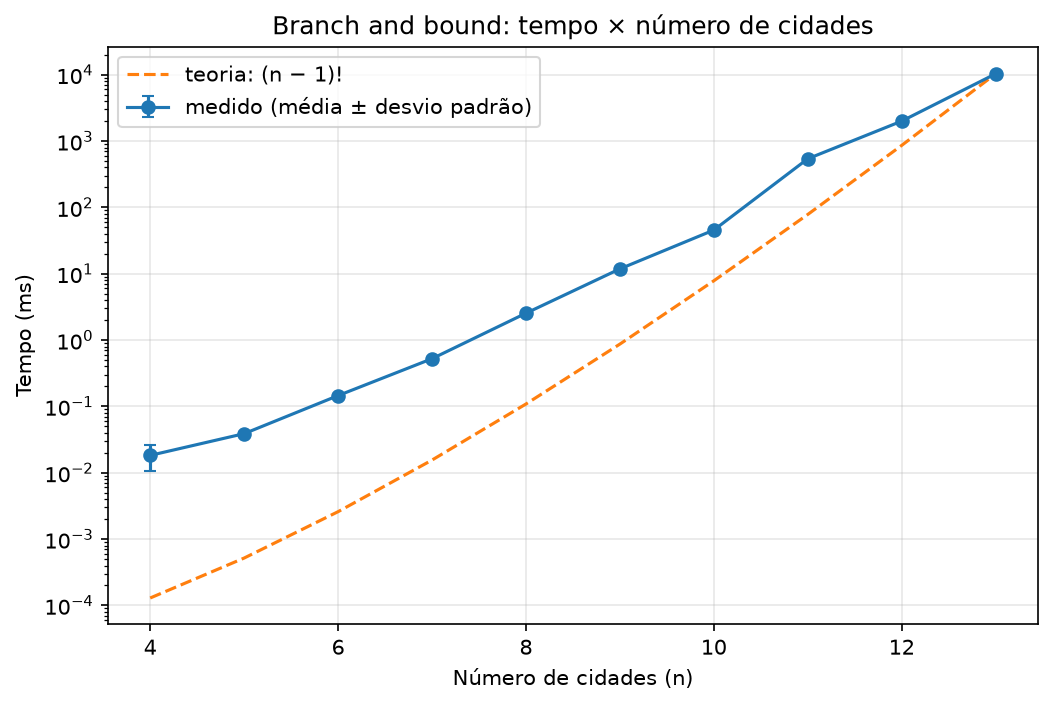
\includegraphics[width=0.78\linewidth]{tempo_bnb.png}
\caption{Tempo do \emph{branch and bound} em função do número de cidades, em escala logarítmica (média $\pm$ desvio padrão de 5 execuções). A curva tracejada é $(n-1)!$, ajustada ao ponto $n = 13$.}
\label{fig:tempobnb}
\end{figure}

A Tabela~\ref{tab:guloso} mostra o custo das rotas do guloso nos tamanhos em que o ótimo é conhecido, e a Figura~\ref{fig:qualidade} resume a diferença percentual. A Figura~\ref{fig:tempoguloso} mostra o tempo do guloso para $n = 4, \dots, 52$, junto com a curva $n^2$ ajustada ao último ponto. Por fim, a Figura~\ref{fig:comparar} compara as rotas dos dois algoritmos com 11 cidades, e a Figura~\ref{fig:guloso52} mostra a rota do guloso nas 52 cidades.

\begin{table}[htbp]
\centering
\caption{Vizinho mais próximo nos tamanhos com ótimo conhecido: custo da rota, ótimo, diferença percentual e tempo (média $\pm$ desvio padrão de 30 execuções).}
\label{tab:guloso}
\small
\begin{tabular}{rrrrr}
\toprule
$n$ & Guloso & Ótimo & Diferença & Tempo (ms) \\
\midrule
 4 & 2598 & 2315 & 12,2\% & 0,0019 $\pm$ 0,0008 \\
 5 & 2607 & 2314 & 12,7\% & 0,0025 $\pm$ 0,0004 \\
 6 & 2608 & 2315 & 12,7\% & 0,0036 $\pm$ 0,0023 \\
 7 & 2632 & 2322 & 13,4\% & 0,0041 $\pm$ 0,0003 \\
 8 & 2902 & 2551 & 13,8\% & 0,0051 $\pm$ 0,0003 \\
 9 & 3198 & 2820 & 13,4\% & 0,0063 $\pm$ 0,0004 \\
10 & 3278 & 2826 & 16,0\% & 0,0076 $\pm$ 0,0023 \\
11 & 4542 & 4038 & 12,5\% & 0,0091 $\pm$ 0,0021 \\
12 & 4560 & 4056 & 12,4\% & 0,0103 $\pm$ 0,0009 \\
13 & 4791 & 4564 &  5,0\% & 0,0121 $\pm$ 0,0020 \\
\midrule
52 & 8980 & 7542$^{*}$ & 19,1\% & 0,1549 $\pm$ 0,0011 \\
\bottomrule
\end{tabular}

\smallskip
{\footnotesize $^{*}$ Ótimo conhecido da TSPLIB; os demais foram obtidos pelo \emph{branch and bound}.}
\end{table}

\begin{figure}[htbp]
\centering
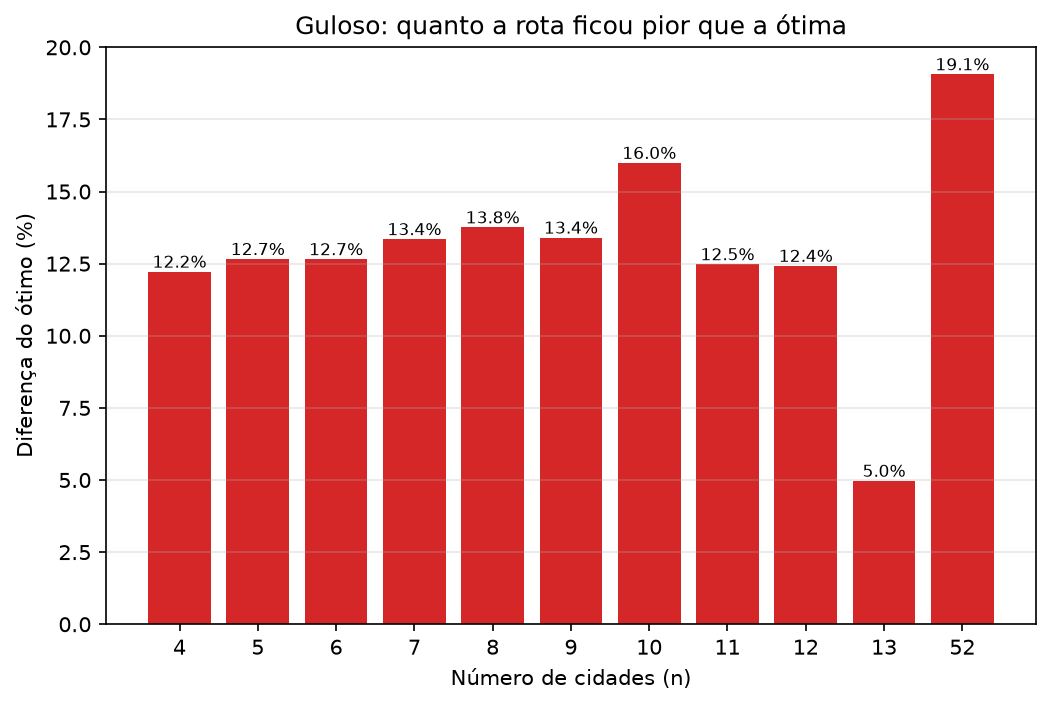
\includegraphics[width=0.78\linewidth]{qualidade_guloso.png}
\caption{Diferença percentual entre o custo da rota do guloso e o ótimo, nos tamanhos em que o ótimo é conhecido.}
\label{fig:qualidade}
\end{figure}

\begin{figure}[htbp]
\centering
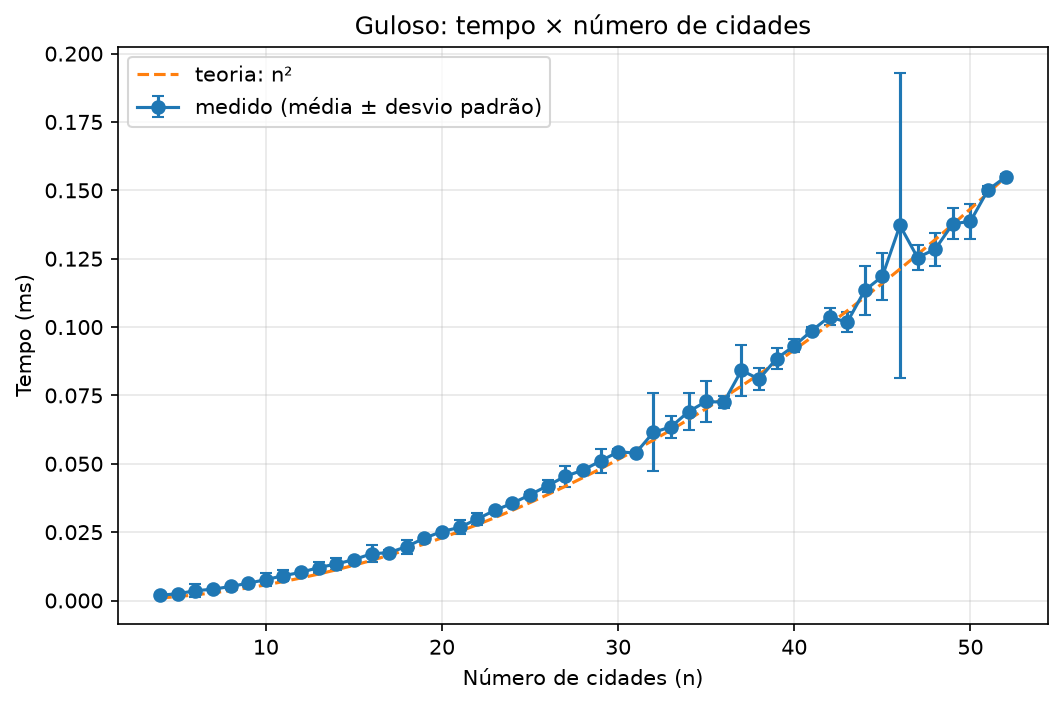
\includegraphics[width=0.78\linewidth]{tempo_guloso.png}
\caption{Tempo do vizinho mais próximo em função do número de cidades (média $\pm$ desvio padrão de 30 execuções). A curva tracejada é $n^2$, ajustada ao ponto $n = 52$.}
\label{fig:tempoguloso}
\end{figure}

\begin{figure}[htbp]
\centering
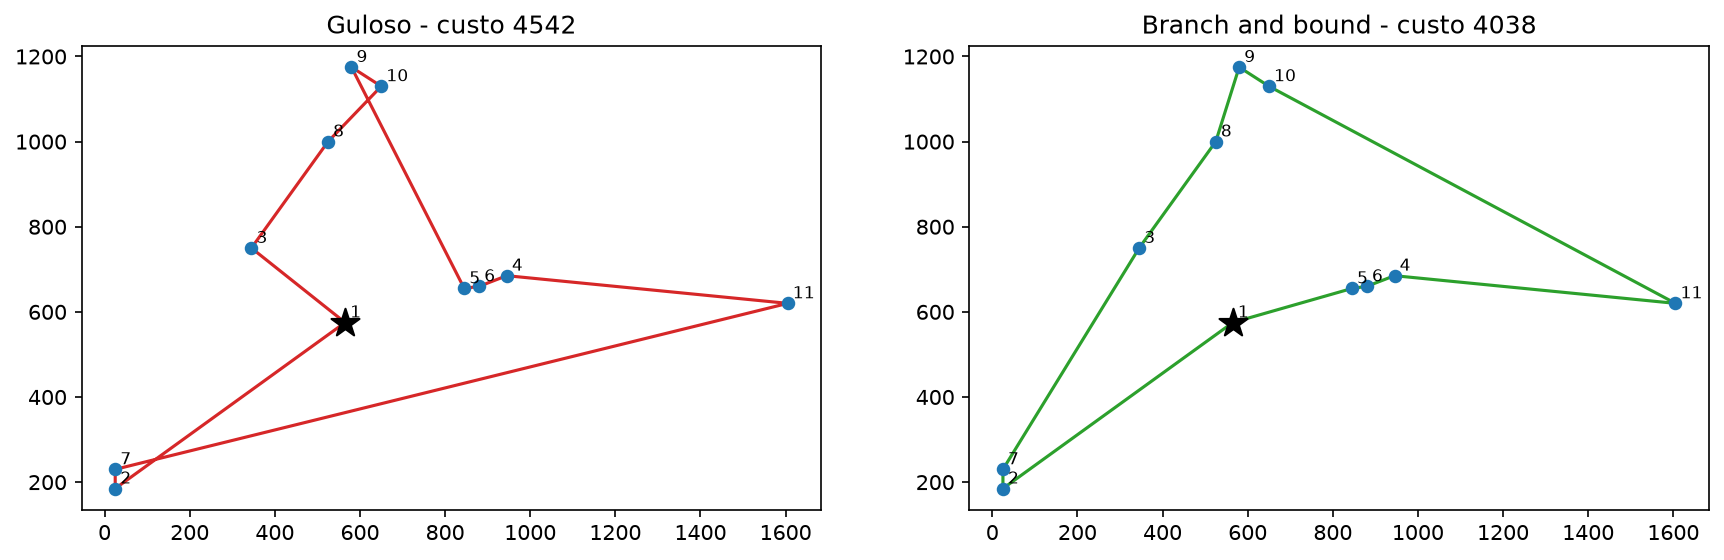
\includegraphics[width=\linewidth]{comparar.png}
\caption{Rotas com as 11 primeiras cidades, partindo da cidade~1 (estrela). À esquerda, o guloso (custo 4542); à direita, a rota ótima encontrada pelo \emph{branch and bound} (custo 4038).}
\label{fig:comparar}
\end{figure}

\begin{figure}[htbp]
\centering
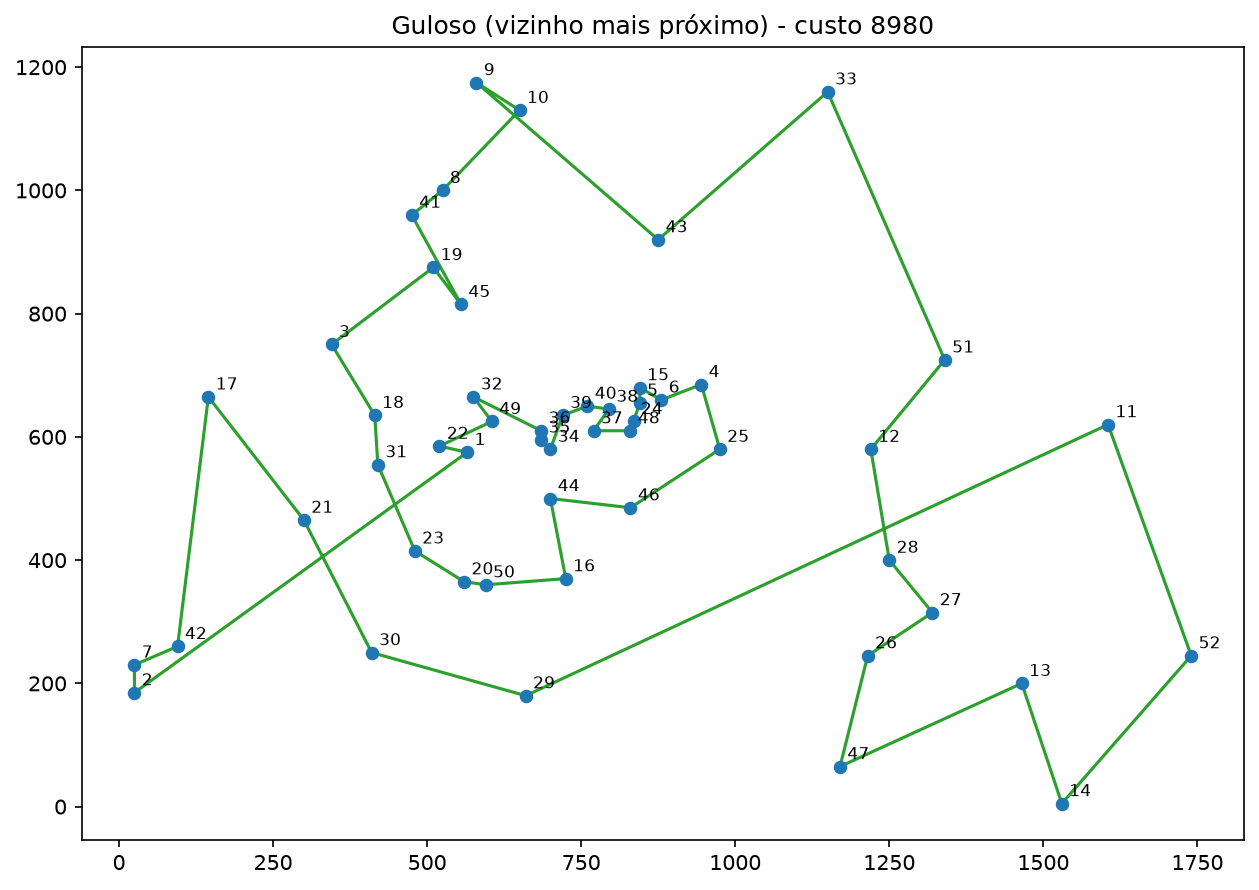
\includegraphics[width=0.85\linewidth]{guloso.png}
\caption{Rota do vizinho mais próximo na berlin52 completa, partindo da cidade~1: custo 8980, 19,1\% acima do ótimo de 7542.}
\label{fig:guloso52}
\end{figure}

% =====================================================================
\section{Discussão}\label{sec:discussao}
% =====================================================================

\paragraph{Guloso: tempo.} O tempo medido acompanha de perto a curva $n^2$ em toda a faixa de 4 a 52 cidades (Figura~\ref{fig:tempoguloso}), como previsto pela análise $\Theta(n^2)$. Com 52 cidades, o guloso levou 0,15\,ms, o equivalente a cerca de 58\,ns por iteração do laço interno. Os poucos pontos com desvio padrão alto, como $n = 46$, são ruído de medição em tempos da ordem de décimos de milissegundo.

\paragraph{Guloso: qualidade.} Em todos os tamanhos com ótimo conhecido, o guloso ficou acima do ótimo, com diferença entre 5,0\% ($n = 13$) e 19,1\% ($n = 52$). A diferença não cresce de forma regular com $n$: ela depende de como as cidades estão dispostas. O padrão do erro, no entanto, é sempre o mesmo, e as Figuras~\ref{fig:comparar} e~\ref{fig:guloso52} o mostram bem: como o guloso não considera os passos seguintes, cidades distantes ficam para o fim, e a rota acaba tendo de atravessar o mapa. Com 11 cidades, a cidade~11, isolada a leste, só é visitada quando restam apenas as cidades 7 e 2, no sudoeste, e a rota precisa da aresta $11 \to 7$, de comprimento 1627, para chegar até elas; a rota ótima chega à cidade~11 a partir da cidade~10 (1083) e sai dela para a cidade~4 (663). Com 52 cidades, o guloso usa a aresta $11 \to 29$ (1042) e fecha o ciclo com a aresta $2 \to 1$ (666). Os 19,1\% acima do ótimo na instância completa são compatíveis com o que a literatura relata para o vizinho mais próximo em instâncias euclidianas aleatórias, com excessos típicos da ordem de 25\%~\cite{johnson1997}.

\paragraph{\emph{Branch and bound}: tempo.} A análise prevê tempo $O(n!)$ no pior caso. Em escala logarítmica, uma curva exponencial aparece como uma reta, e a fatorial, como uma curva cada vez mais inclinada. Os tempos medidos ficam próximos de uma reta (Figura~\ref{fig:tempobnb}): o tempo cresceu, em média, 4,4 vezes a cada cidade acrescentada (média geométrica entre $n = 4$ e $n = 13$), enquanto $(n-1)!$ cresce $n - 1$ vezes, ou seja, 12 vezes ao passar de 12 para 13 cidades. A diferença se deve à poda: a fração da árvore efetivamente visitada caiu de 100\% com 4 cidades para 1,7\% com 13 (Tabela~\ref{tab:bnb}). Como a curva teórica foi ajustada ao ponto $n = 13$ e cresce mais rápido que a medida, ela fica abaixo dos tempos medidos para $n$ menores. As medições não contradizem o limite $O(n!)$, que vale para o pior caso; elas mostram que, nesta instância, a poda reduz bastante o fator de crescimento, embora o tempo continue exponencial.

O efeito da poda depende também da instância, e não só de $n$. A passagem de 10 para 11 cidades multiplicou o tempo por 11,9, bem acima da média, e a fração visitada da árvore subiu de 9,7\% para 11,3\%. A cidade~11 fica isolada, longe das demais (Figura~\ref{fig:comparar}), e o ótimo saltou de 2826 para 4038. Enquanto um caminho parcial não passa pela cidade~11, o seu custo subestima muito o custo da rota completa, de modo que o limitante usado, o custo parcial, só consegue podar tarde.

\paragraph{Maior tamanho resolvido.} O B\&B resolveu até 13 cidades em cerca de 10\,s por execução. Extrapolando o fator médio de 4,4 por cidade, 14 cidades levariam cerca de 45\,s; 15 cidades, cerca de 3\,min; 16 cidades, cerca de 14\,min; e 20 cidades, cerca de 3,5 dias. Essas extrapolações são apenas estimativas, pois o fator varia com a instância, mas deixam claro que as 52 cidades da berlin52 estão fora de alcance. O guloso, por sua vez, resolve as 52 cidades em 0,15\,ms. Com 13 cidades, o B\&B foi cerca de 850 mil vezes mais lento que o guloso, em troca de eliminar uma diferença de 5,0\% no custo da rota.

\paragraph{Combinação dos dois algoritmos.} Usar o guloso como limite inicial do B\&B mostrou-se vantajoso: o guloso custa $\Theta(n^2)$, desprezível perto do B\&B, e fornece desde o início uma rota de referência que permite podar. Sem ela, a poda só começaria depois que a busca chegasse à primeira rota completa.

% =====================================================================
\section{Conclusão}\label{sec:conclusao}
% =====================================================================

Este trabalho comparou um algoritmo exato e uma heurística para o PCV simétrico. A análise teórica previu tempo $\Theta(n^2)$ para o vizinho mais próximo e $O(n!)$ para o \emph{branch and bound}, e os experimentos confirmaram a diferença na prática: o guloso resolveu as 52 cidades da berlin52 em 0,15\,ms, enquanto o B\&B ficou limitado a 13 cidades, em cerca de 10\,s. Em contrapartida, só o B\&B garante a rota ótima. O guloso ficou entre 5\% e 19\% acima dela, e o contraexemplo com quatro cidades mostra que a falha vem da própria estratégia de nunca rever uma escolha.

O principal aprendizado é que o tamanho do espaço de soluções domina todo o resto: com 13 cidades, a poda eliminou mais de 98\% da árvore e, ainda assim, cada cidade a mais multiplicou o tempo por cerca de 4. Para resolver instâncias maiores, é preciso melhorar o limitante, e não apenas a implementação.

Como trabalhos futuros, propomos: (i) usar limitantes inferiores mais fortes no B\&B, como o custo de uma árvore geradora mínima sobre as cidades restantes ou a redução de matriz de Little et al.~\cite{little1963}; (ii) ordenar os filhos de cada nó pela distância, para encontrar boas rotas mais cedo; (iii) eliminar a simetria de sentido, que hoje faz cada ciclo aparecer duas vezes na árvore; (iv) comparar o B\&B com a programação dinâmica de Held e Karp~\cite{heldkarp1962}, de tempo $O(n^2 2^n)$; (v) melhorar a rota do guloso com busca local, como o 2-opt, ou executá-lo a partir de cada cidade inicial e guardar a melhor rota; e (vi) repetir os experimentos nas instâncias st70 e pr76 da TSPLIB.

% =====================================================================
\begin{thebibliography}{99}
% =====================================================================

\bibitem{applegate2006}
APPLEGATE, D. L.; BIXBY, R. E.; CHVÁTAL, V.; COOK, W. J.
\emph{The Traveling Salesman Problem: A Computational Study}.
Princeton: Princeton University Press, 2006.

\bibitem{cormen2009}
CORMEN, T. H.; LEISERSON, C. E.; RIVEST, R. L.; STEIN, C.
\emph{Introduction to Algorithms}. 3.~ed.
Cambridge: MIT Press, 2009.

\bibitem{enunciado}
\pendente{SOBRENOME, Nome do professor}.
\emph{Enunciado do trabalho prático de Projeto e Análise de Algoritmos}.
\pendente{Instituição}, 2026.

\bibitem{garey1979}
GAREY, M. R.; JOHNSON, D. S.
\emph{Computers and Intractability: A Guide to the Theory of NP-Completeness}.
San Francisco: W. H. Freeman, 1979.

\bibitem{heldkarp1962}
HELD, M.; KARP, R. M.
A dynamic programming approach to sequencing problems.
\emph{Journal of the Society for Industrial and Applied Mathematics}, v.~10, n.~1, p.~196--210, 1962.

\bibitem{johnson1997}
JOHNSON, D. S.; McGEOCH, L. A.
The traveling salesman problem: a case study in local optimization.
In: AARTS, E. H. L.; LENSTRA, J. K. (Ed.).
\emph{Local Search in Combinatorial Optimization}.
Chichester: John Wiley \& Sons, 1997. p.~215--310.

\bibitem{karp1972}
KARP, R. M.
Reducibility among combinatorial problems.
In: MILLER, R. E.; THATCHER, J. W. (Ed.).
\emph{Complexity of Computer Computations}.
New York: Plenum Press, 1972. p.~85--103.

\bibitem{land1960}
LAND, A. H.; DOIG, A. G.
An automatic method of solving discrete programming problems.
\emph{Econometrica}, v.~28, n.~3, p.~497--520, 1960.

\bibitem{little1963}
LITTLE, J. D. C.; MURTY, K. G.; SWEENEY, D. W.; KAREL, C.
An algorithm for the traveling salesman problem.
\emph{Operations Research}, v.~11, n.~6, p.~972--989, 1963.

\bibitem{papadimitriou1977}
PAPADIMITRIOU, C. H.
The Euclidean travelling salesman problem is NP-complete.
\emph{Theoretical Computer Science}, v.~4, n.~3, p.~237--244, 1977.

\bibitem{reinelt1991}
REINELT, G.
TSPLIB---A traveling salesman problem library.
\emph{ORSA Journal on Computing}, v.~3, n.~4, p.~376--384, 1991.

\bibitem{rosenkrantz1977}
ROSENKRANTZ, D. J.; STEARNS, R. E.; LEWIS, P. M.
An analysis of several heuristics for the traveling salesman problem.
\emph{SIAM Journal on Computing}, v.~6, n.~3, p.~563--581, 1977.

\end{thebibliography}

\end{document}
